%\documentclass[notes]{beamer}       % print frame + notes
%documentclass[notes=only]{beamer}   % only notes
\documentclass{beamer}              % only frames

\usetheme{Copenhagen}
\usecolortheme{beaver}

\setbeamertemplate{navigation symbols}{}

\setbeamertemplate{frametitle}[default][center]

\usepackage{biblatex}
\bibliography{main}

\usepackage{hyperref}
\usepackage{minted}
\usepackage{amsmath}
\usepackage{multicol}
\usepackage{bibentry}

\usepackage{graphicx}
\usepackage{tikz}

\usetikzlibrary{calc, patterns}

\title{Evolutionary Game Theory}
\author{Vince Knight}
\date{}


\begin{document}

\frame{
    \titlepage
}

\section{knightva@cardiff.ac.uk}

\begin{frame}
    \centering

    
\includegraphics[height=2cm]{static/CUident_CMYK.png}
    \hfill
    
\includegraphics[height=2cm]{static/Logo_UNAM_Namibia.png}\\
    \tiny{2024-03-04 until 2024-03-29}

\end{frame}

\begin{frame}
    \centering

    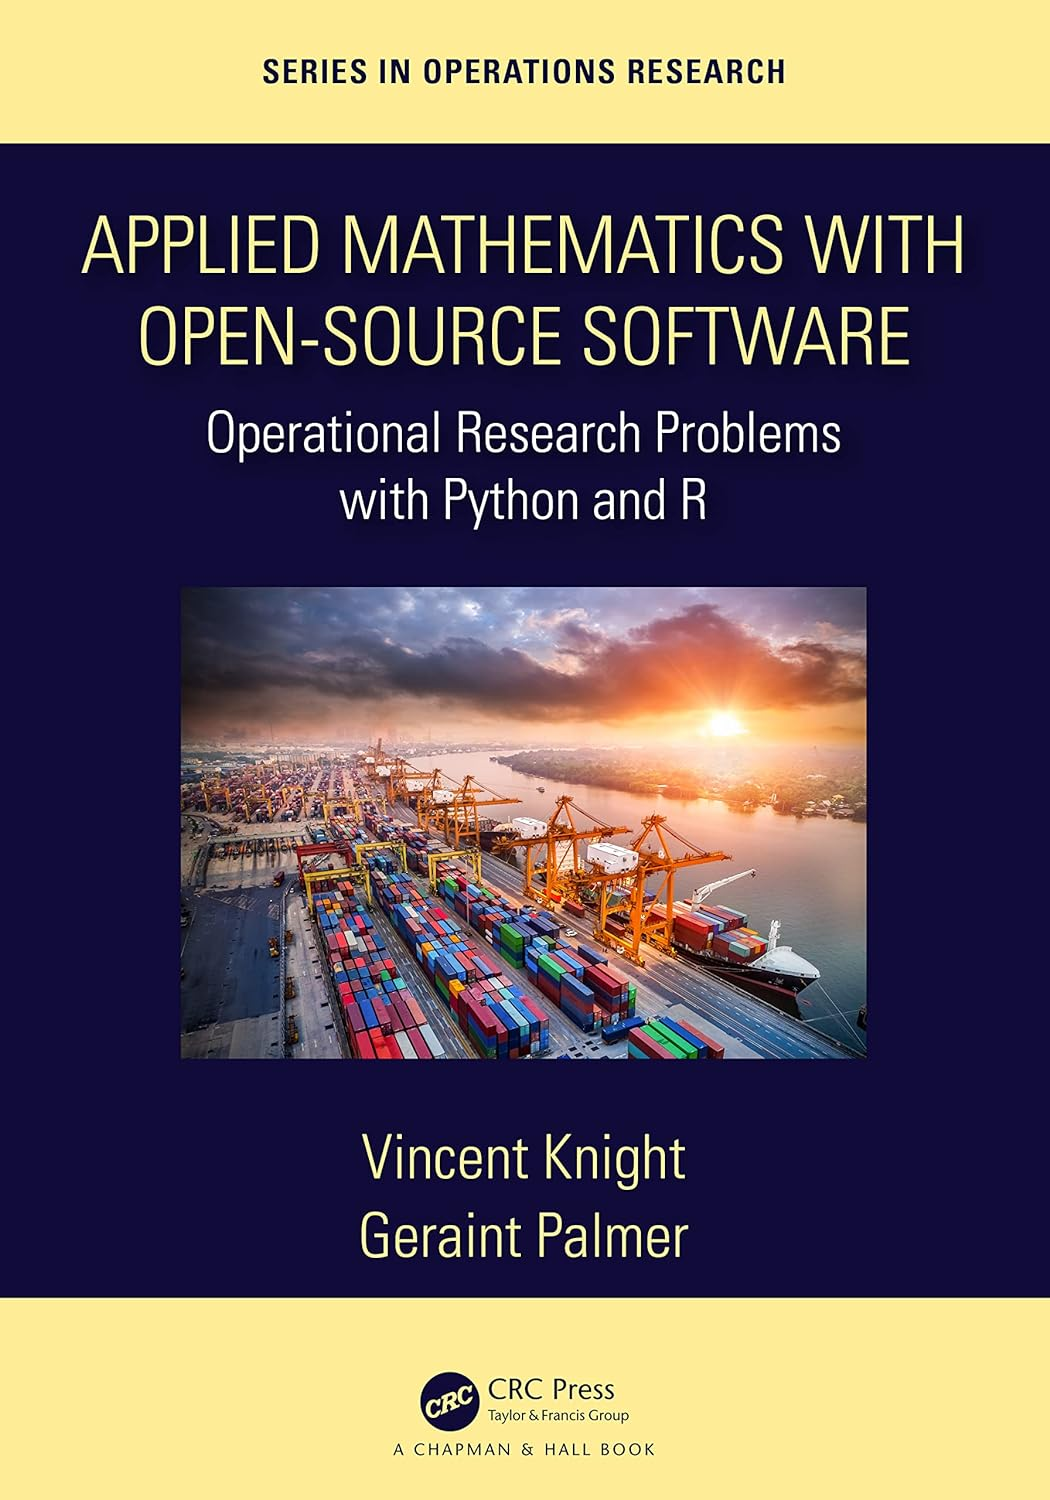
\includegraphics[height=5cm]{static/book.jpg}
    \hfill
    
\includegraphics[height=5cm]{static/nash-street.jpg}
\end{frame}

\section{Population Games}

\begin{frame}
    \frametitle{Two Thirds of the Average}
        \begin{alertblock}{}
            \centering
            \begin{itemize}
                \item Pick an integer between 0 and 100 (inclusive);
                \item Closest to two thirds of the average of all picked numbers wins.
            \end{itemize}
        \end{alertblock}
\end{frame}

\note{
    If we consider all possible strategies the game is equivalent to picking a
    number on this line:

    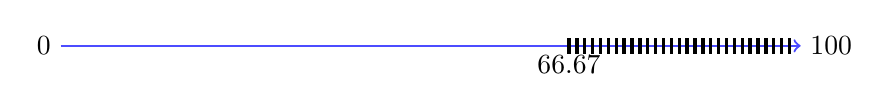
\begin{tikzpicture}
        \node (0) at (0, 0) {0};
        \node (100) at (10, 0) {100};
        \draw [->, thick, blue!70] (0) to (100);
        \node [below] (66) at (6.67, 0) {66.67};

        \foreach \x in {6.67,6.77,...,9.57}
        {
            \draw [very thick, black] (\x, -.1) to (\x, .1);
        }
    \end{tikzpicture}
    The biggest possible winning guess is \(2\frac{100}{3}\approx 66.67\) which
    only occurs if all other guesses are larger than that.

    Thus all choices bigger than \(2\frac{100}{3}\) are \textbf{dominated}. If
    we continue to repeat this process we see that there are only two valid
    equilibrium:

    \begin{itemize}
        \item All players guess 0.
        \item All players guess 1.
    \end{itemize}

    Now that we have rationalised this behaviour, let us play again.
}


\begin{frame}
    \begin{center}
        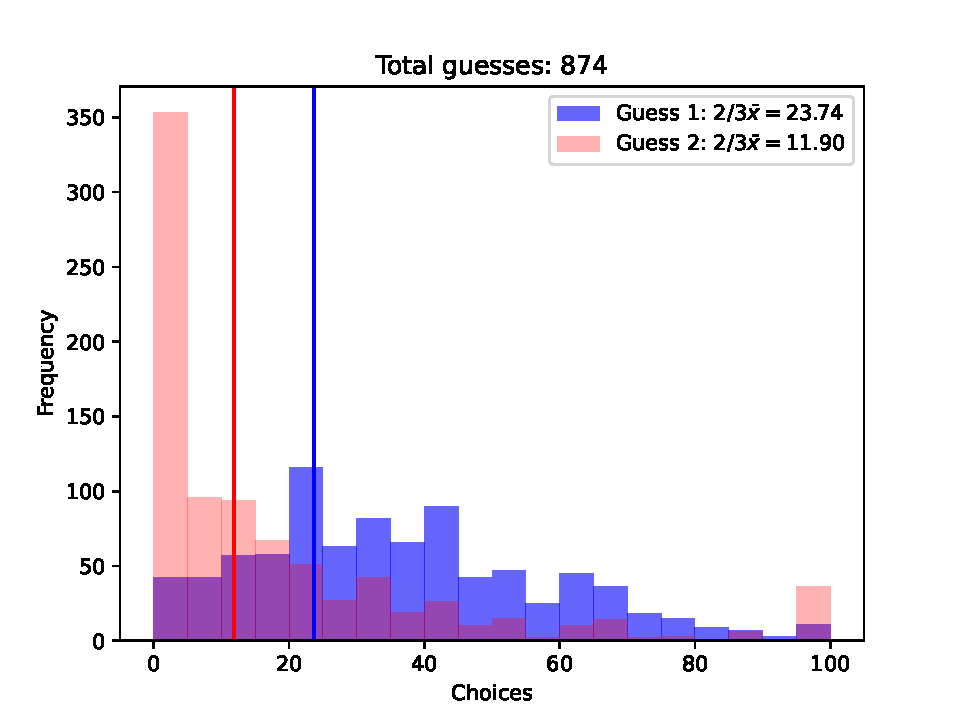
\includegraphics[width=.8\textwidth]{./static/two_thirds_of_the_average_game/history_of_play/main.pdf}
    \end{center}
\end{frame}

\note{
    We see that over the two guesses the behaviour shifts.

    Note that with the first guesses: most people were above the winning guess.

    For the second guess: most people were below the winning guess.

    Will we eventually arrive at the equilibrium?
}

\begin{frame}
    \begin{center}
        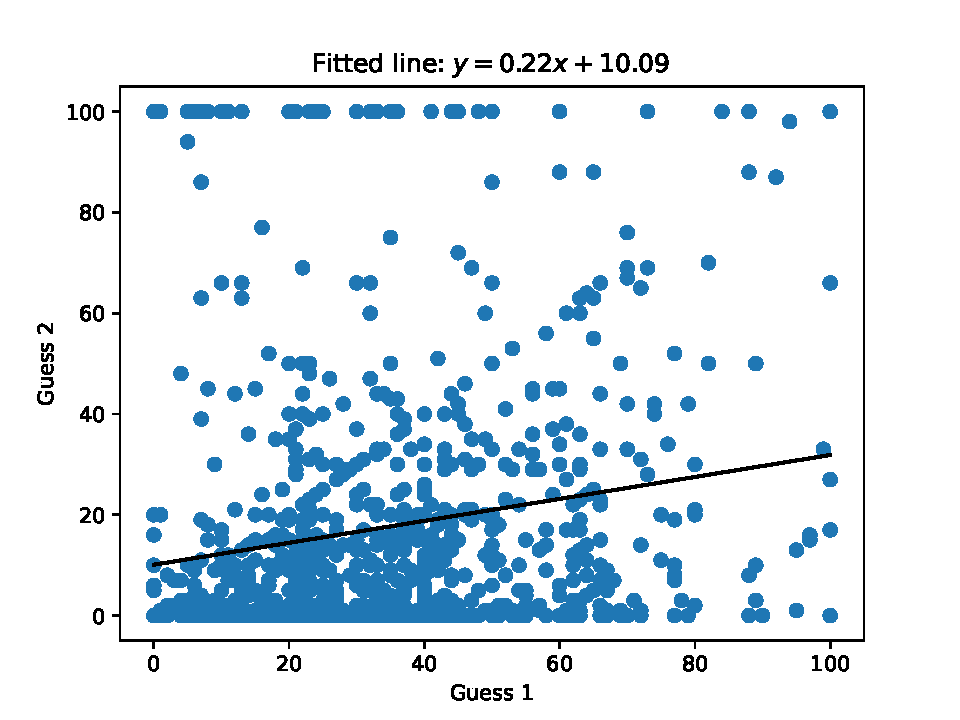
\includegraphics[width=.8\textwidth]{./static/two_thirds_of_the_average_game/linear_regression_of_play/main.pdf}
    \end{center}
\end{frame}

\note{
    One approach would be to model the macro behaviour with that fitted line: if
    we assume that the $n+1$th guess is $.22$ of the $n$th guess we could
    imagine that this would eventually converge. We'd need more data here of
    course.

    This does not necessarily work, perhaps, as most players in the second guess
    were below the winning guess, a third guess would in fact be higher! So
    perhaps the linear regression would not longer be accurate.

    Let us base our analysis on biological evolution.
}

\begin{frame}
    \begin{definition}
        Considering an infinite population of individuals each of which
        represents an action from $\mathcal{A}$, we define the population profile
        as a vector $x\in[0,1]^{|\mathcal{A}|}_\mathbb{R}$. Note that:

        $$\sum_{i\in \mathcal{A}}x_i=1$$
    \end{definition}
\end{frame}

\note{
    For the two thirds game, our vector \(x \in \mathbb{R}_{[0, 1]}^{101}\).

    Now: for evolution we need fitness.
}

\begin{frame}
    \begin{definition}
        The population dependent fitness of an individual of type \(i\) in a
        population \(x\) is denoted as \(f_i: \mathbb{R}_{[0, 1]}^{101} \to
        \mathbb{R} \).
    \end{definition}
\end{frame}

\note{
    For two thirds game a sensible fitness function would be something inversely
    proportional to the winning guess:

    \[
        f_i(x) = \frac{1}{1 + \left(i - \frac{2}{3}\sum_{i=0}^{N}ix_i\right) ^ 2}
    \]

    \textbf{Note} we add 1 to the denominator to deal with division by zero
    that can occur in some populations.

    Now we need an equation to model the evolutionary process.
}

\section{Replicator dynamics}

\begin{frame}
    \begin{definition}{Replicator Dynamics Equation}
        \[\frac{dx_i}{dt}=x_i(f_i(x) - \phi)\text{ for all }i\]

        where: 

        \[\phi=\sum_{i=0}^Nx_if_i(x)\]
    \end{definition}
\end{frame}

\note{
    This differential equation ensures that individuals with a fitness above
    the average \(\phi\) have positive derivative and individuals with a fitness
    below the average \(\phi\) have negative derivate.

    For the case of the two thirds game we can solve the differential equations
    numerically efficiently.

}

\begin{frame}
    \begin{center}
        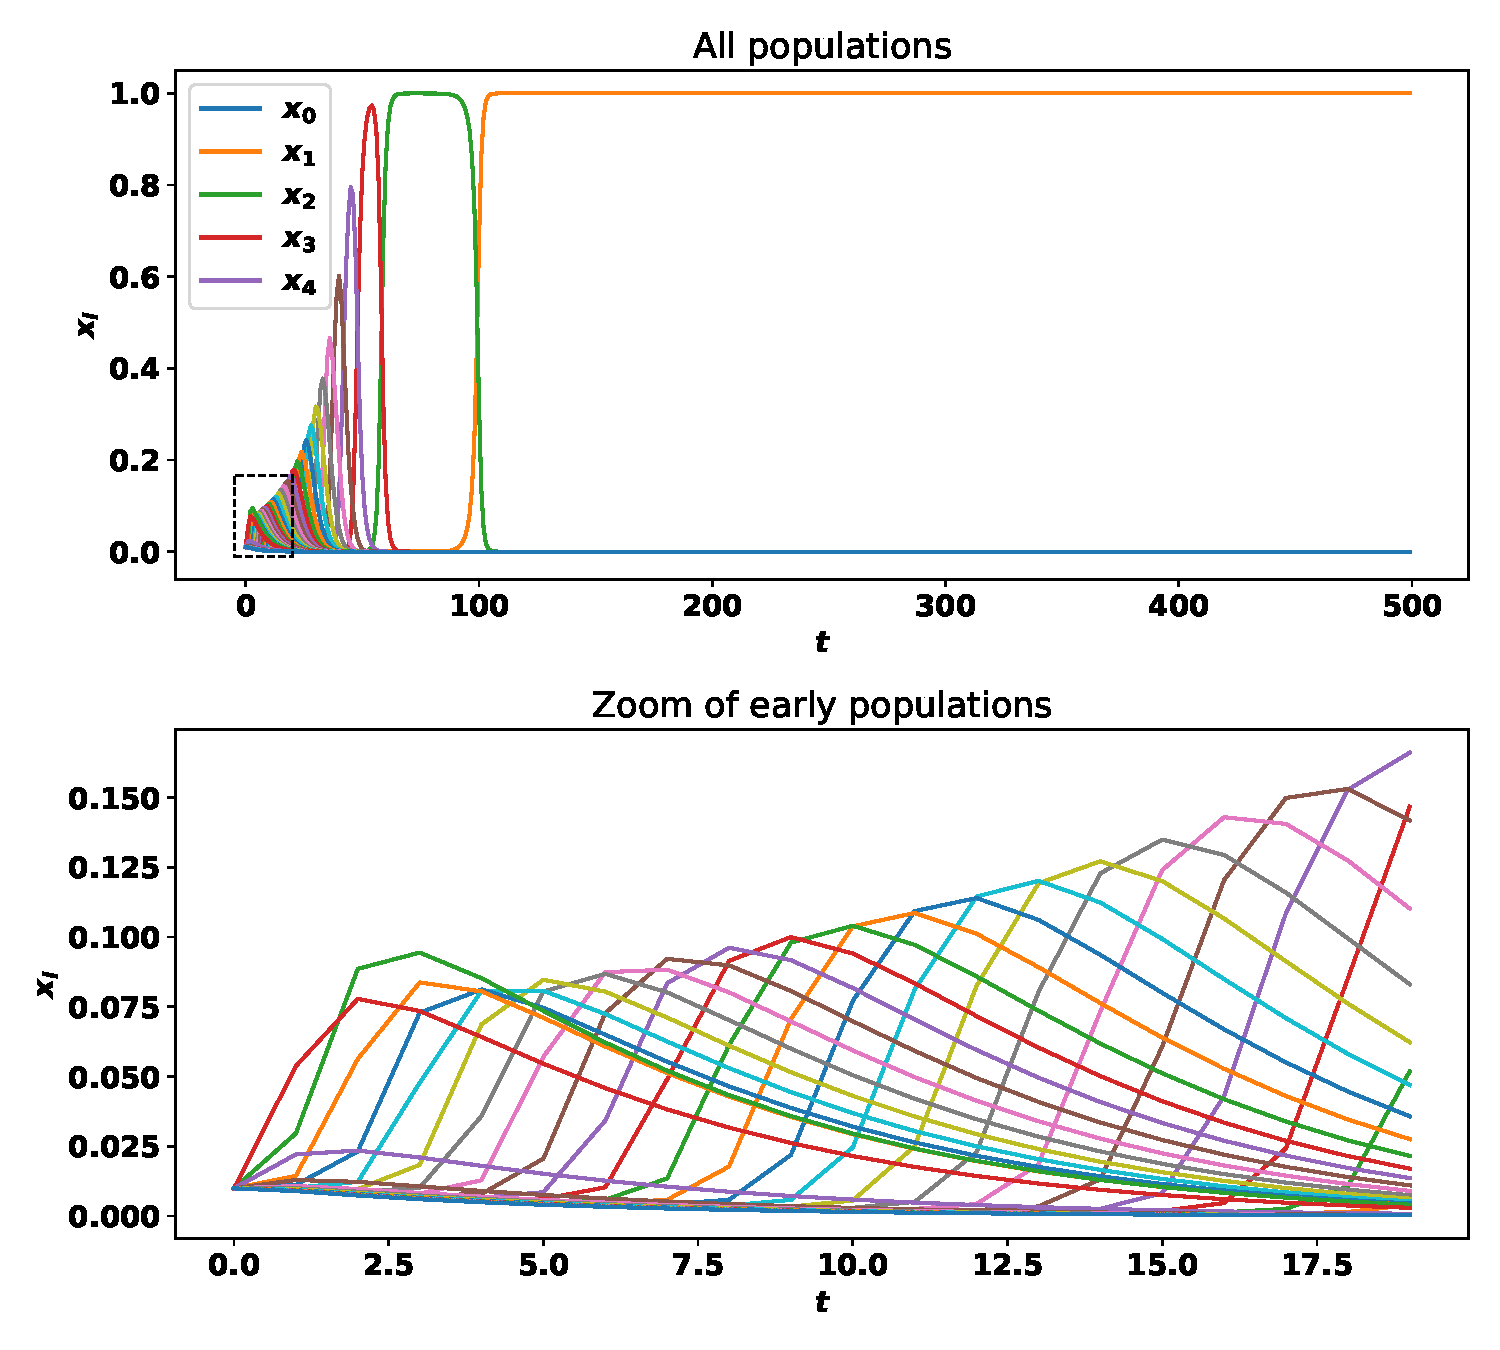
\includegraphics[width=.8\textwidth]{./static/two_thirds_of_the_average_game/numerical_solution_of_replicator_dynamics/main.pdf}
    \end{center}
\end{frame}

\begin{frame}
    We see that over time, the population emerges to all guessing 1. So everyone
    wins.

     Note that everyone guessing 0 also is stable. 
\end{frame}

\begin{frame}
    \begin{center}
        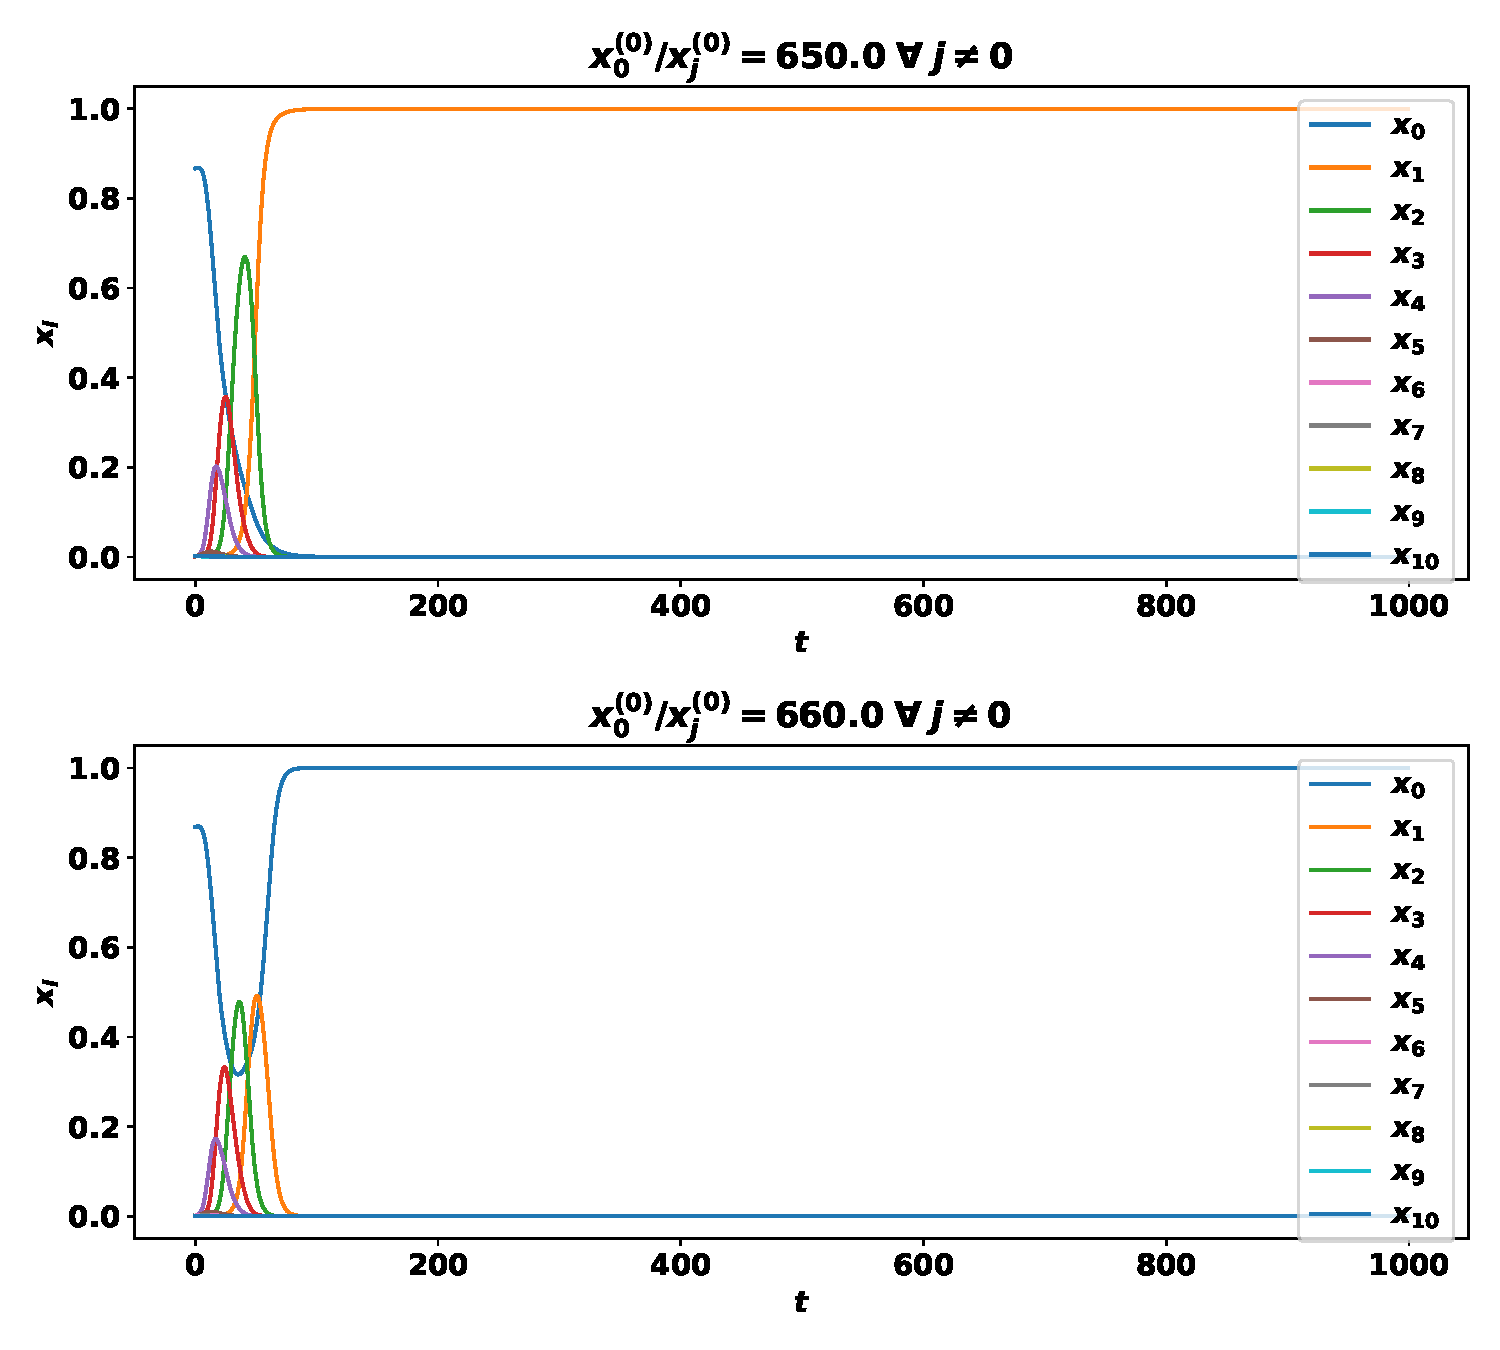
\includegraphics[width=.8\textwidth]{./static/two_thirds_of_the_average_game/numerical_solution_of_replicator_dynamics_with_different_starting_populations/main.pdf}
    \end{center}
\end{frame}

\note{
With a different starting population we can also emerge to that stable
population.

Both these populations are stable.
}

\section{Evolutionary Stable Strategies}


\frame{
    \centering
    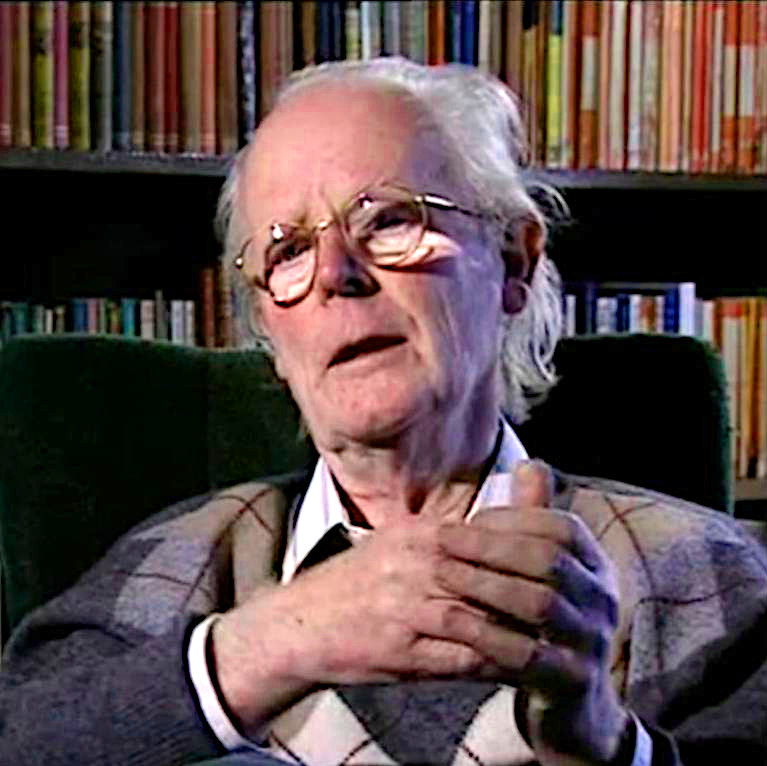
\includegraphics[height=.6\textheight]{./static/maynard-smith.jpg}

    \textbf{John Maynard-Smith}\footfullcite{smith1977theory} (1920 - 2004)

    \tiny{By Web of Stories - Web of Stories, CC BY-SA 3.0, https://commons.wikimedia.org/w/index.php?curid=20096037}

}

\note{
    This leads to John Maynard-Smith. He is often considered the father of
    evolutionary game theory.

    He defined the concept of an Evolutionary Stable Strategy.

    We will use the concept of a particular type of evolutionary game to
    describe this.
}

\begin{frame}
    \begin{definition}
        In a population game when considering a pairwise contest game we assume
        that individuals are randomly matched and play some game with utility
        matrices \(A, A^{T}\). For a population profile \(x\) this gives a compact
        expression for the fitness:

        \[f=Ax\]

    \end{definition}
\end{frame}

\note{
    As an example, let us consider the Hawk Dove game which is attributed to
    Maynard-Smith. Two types of behaviour: 
    \(\{\text{Aggressive}, \text{Not Aggressive}\}\) referred to as Hawk or
    Dove.


    \begin{itemize}
        \item If a Dove and Hawk meet the Hawk takes the resources getting a utility
            of \(v\), the dove gets \(0\).
        \item If two Doves meet they share the resources both getting \(\frac{v}{2}\)
        \item If two Hawks meet there is a fight over the resources (with an equal chance of winning) 
             and the winner takes the resources while the loser pays a cost
             \(c>v\)
    \end{itemize}

    This corresponds to:

    \[
        A =
        \begin{pmatrix}
            \frac{v-c}{2}&v\\
            0 & \frac{v}{2}
        \end{pmatrix}
    \]
}

\begin{frame}
    \begin{definition}
        In a pairwise interaction game the fitness of a strategy \(\sigma\) in a
        population \(x\) is given by:

        \[u(\sigma, x)=\sum_{i=1}^{\mathcal{|A|}}\sigma_i f_i(x)\]
    \end{definition}
\end{frame}

\note{
    This extension of the notion of fitness allows us to consider individuals as
    strategies. Perhaps more precisely strategies as individuals.

    In this case we can relate evolutionary stability to a subset of Nash
    equilibria which is where we are going.
}

\begin{frame}
    \begin{definition}
        A strategy $\sigma^*$ is called an \textbf{Evolutionary Stable Strategy}
        if there exists an $0<\bar\epsilon<1$ such that for every
        $0<\epsilon<\bar \epsilon$ and every $\sigma\ne \sigma^*$
        $\sigma^*$ is:

        $$u(\sigma^*, x_\epsilon)>u(\sigma, x_\epsilon)$$

        Where \(x_\epsilon\) is the post entry population where a proportion
        \(\epsilon\) of the population are \(\sigma\).
    \end{definition}
\end{frame}

\note{
    This corresponds to the idea that for a small enough change of the
    population that an evolutionary stable strategy will reject the change.

    This is similar to what we discussed with the two thirds of the average
    game.

    The strategy 0 would be considered to be evolutionarily stable because there
    exists a small enough change of the population from everyone playing 0 that
    returns to everyone playing 0.
}

\frame{
    \begin{center}
        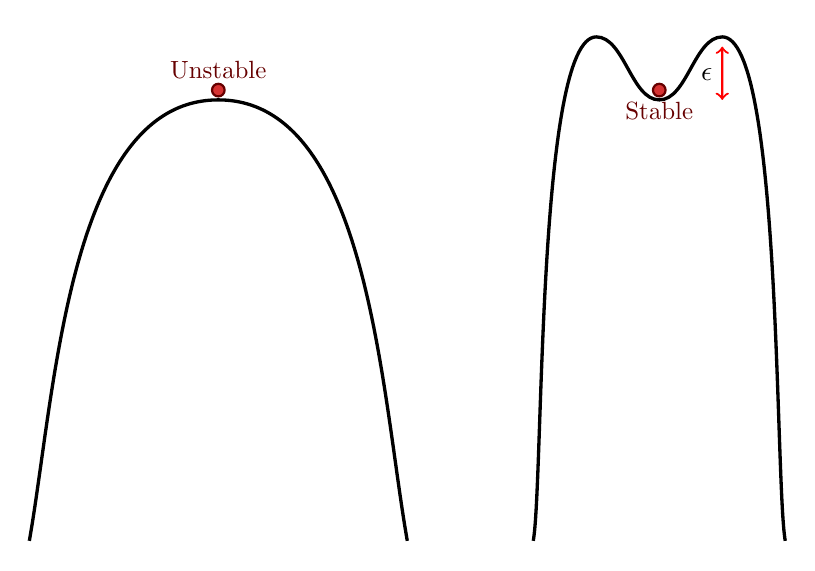
\begin{tikzpicture}[scale=.8]
            \node (unstable) at (0, 0) {};
            \draw [very thick, black] (-3, -7) 
                to[out=80,in=180,looseness=0.8] (unstable.center)
                to[out=0,in=100,looseness=0.8] (3, -7);
            \draw [thick, red!40!black,fill=red!80!black!80] (unstable.north)
                  circle(0.1) 
                  node[above=1,scale=0.9] {Unstable};

            \node (stable) at (7, 0) {};
            \node (A) at (6, 1) {};
            \node (B) at (8, 1) {};
            \draw [very thick, black] (5, -7) 
                to[out=80, in=180, looseness=.3] (A.center)
                to[out=0,in=180,looseness=0.8] (stable.center)
                to[out=0, in=180, looseness=.8] (B.center)
                to[out=0,in=100,looseness=0.3] (9, -7);
            \draw [thick, red!40!black,fill=red!80!black!80] (stable.north)
                  circle(0.1) 
                  node[below=1,scale=0.9] {Stable};

            \draw [thick, red, <->] (B.south) to (8, 0);
            \node [anchor=east] at (8, .4) {\(\epsilon\)};

        \end{tikzpicture}
    \end{center}
}

\note{
    This corresponds to the idea of both of those two pictures are stable.
    However, only one of them can be pushed with \textbf{any} force without the
    marble falling.
}

\frame{
    \begin{theorem}

        If \(\sigma^*\) is an ESS in a pairwise contest population game then for
        all \(\sigma\ne\sigma^*\):

        1. \(u(\sigma^*,\sigma^*)>u(\sigma,\sigma^*)\)
        OR
        2. \(u(\sigma^*,\sigma^*)=u(\sigma,\sigma^*)\) and \(u(\sigma^*,\sigma)>u(\sigma,\sigma)\)

        Conversely, if either (1) or (2) holds for all \(\sigma\ne\sigma^*\) in
        a two player normal form game then \(\sigma^*\) is an ESS.
    \end{theorem}
}

\note{
This result gives us an efficient way of computing ESS. The first condition is in fact almost a condition for Nash Equilibrium (with a strict inequality), the second is thus a stronger condition that removes certain Nash equilibria from consideration. This becomes particularly relevant when considering Nash equilibrium in mixed strategies.

To find ESS in a pairwise context population game we:

\begin{enumerate}
    \item Write down the associated two-player game;
    \item Identify all symmetric Nash equilibria of the game;
    \item Test the Nash equilibrium against the two conditions of the Theorem.
\end{enumerate}

For the Hawk-Dove game this can be used to show that
\(\sigma^*=(\frac{v}{c},1-\frac{v}{c})\) is an ESS.

}


\frame{
    \begin{block}{}
        An evolutionary game theoretic model of rhino horn devaluation\footfullcite{glynatsi2018}
    \end{block}
    \centering
    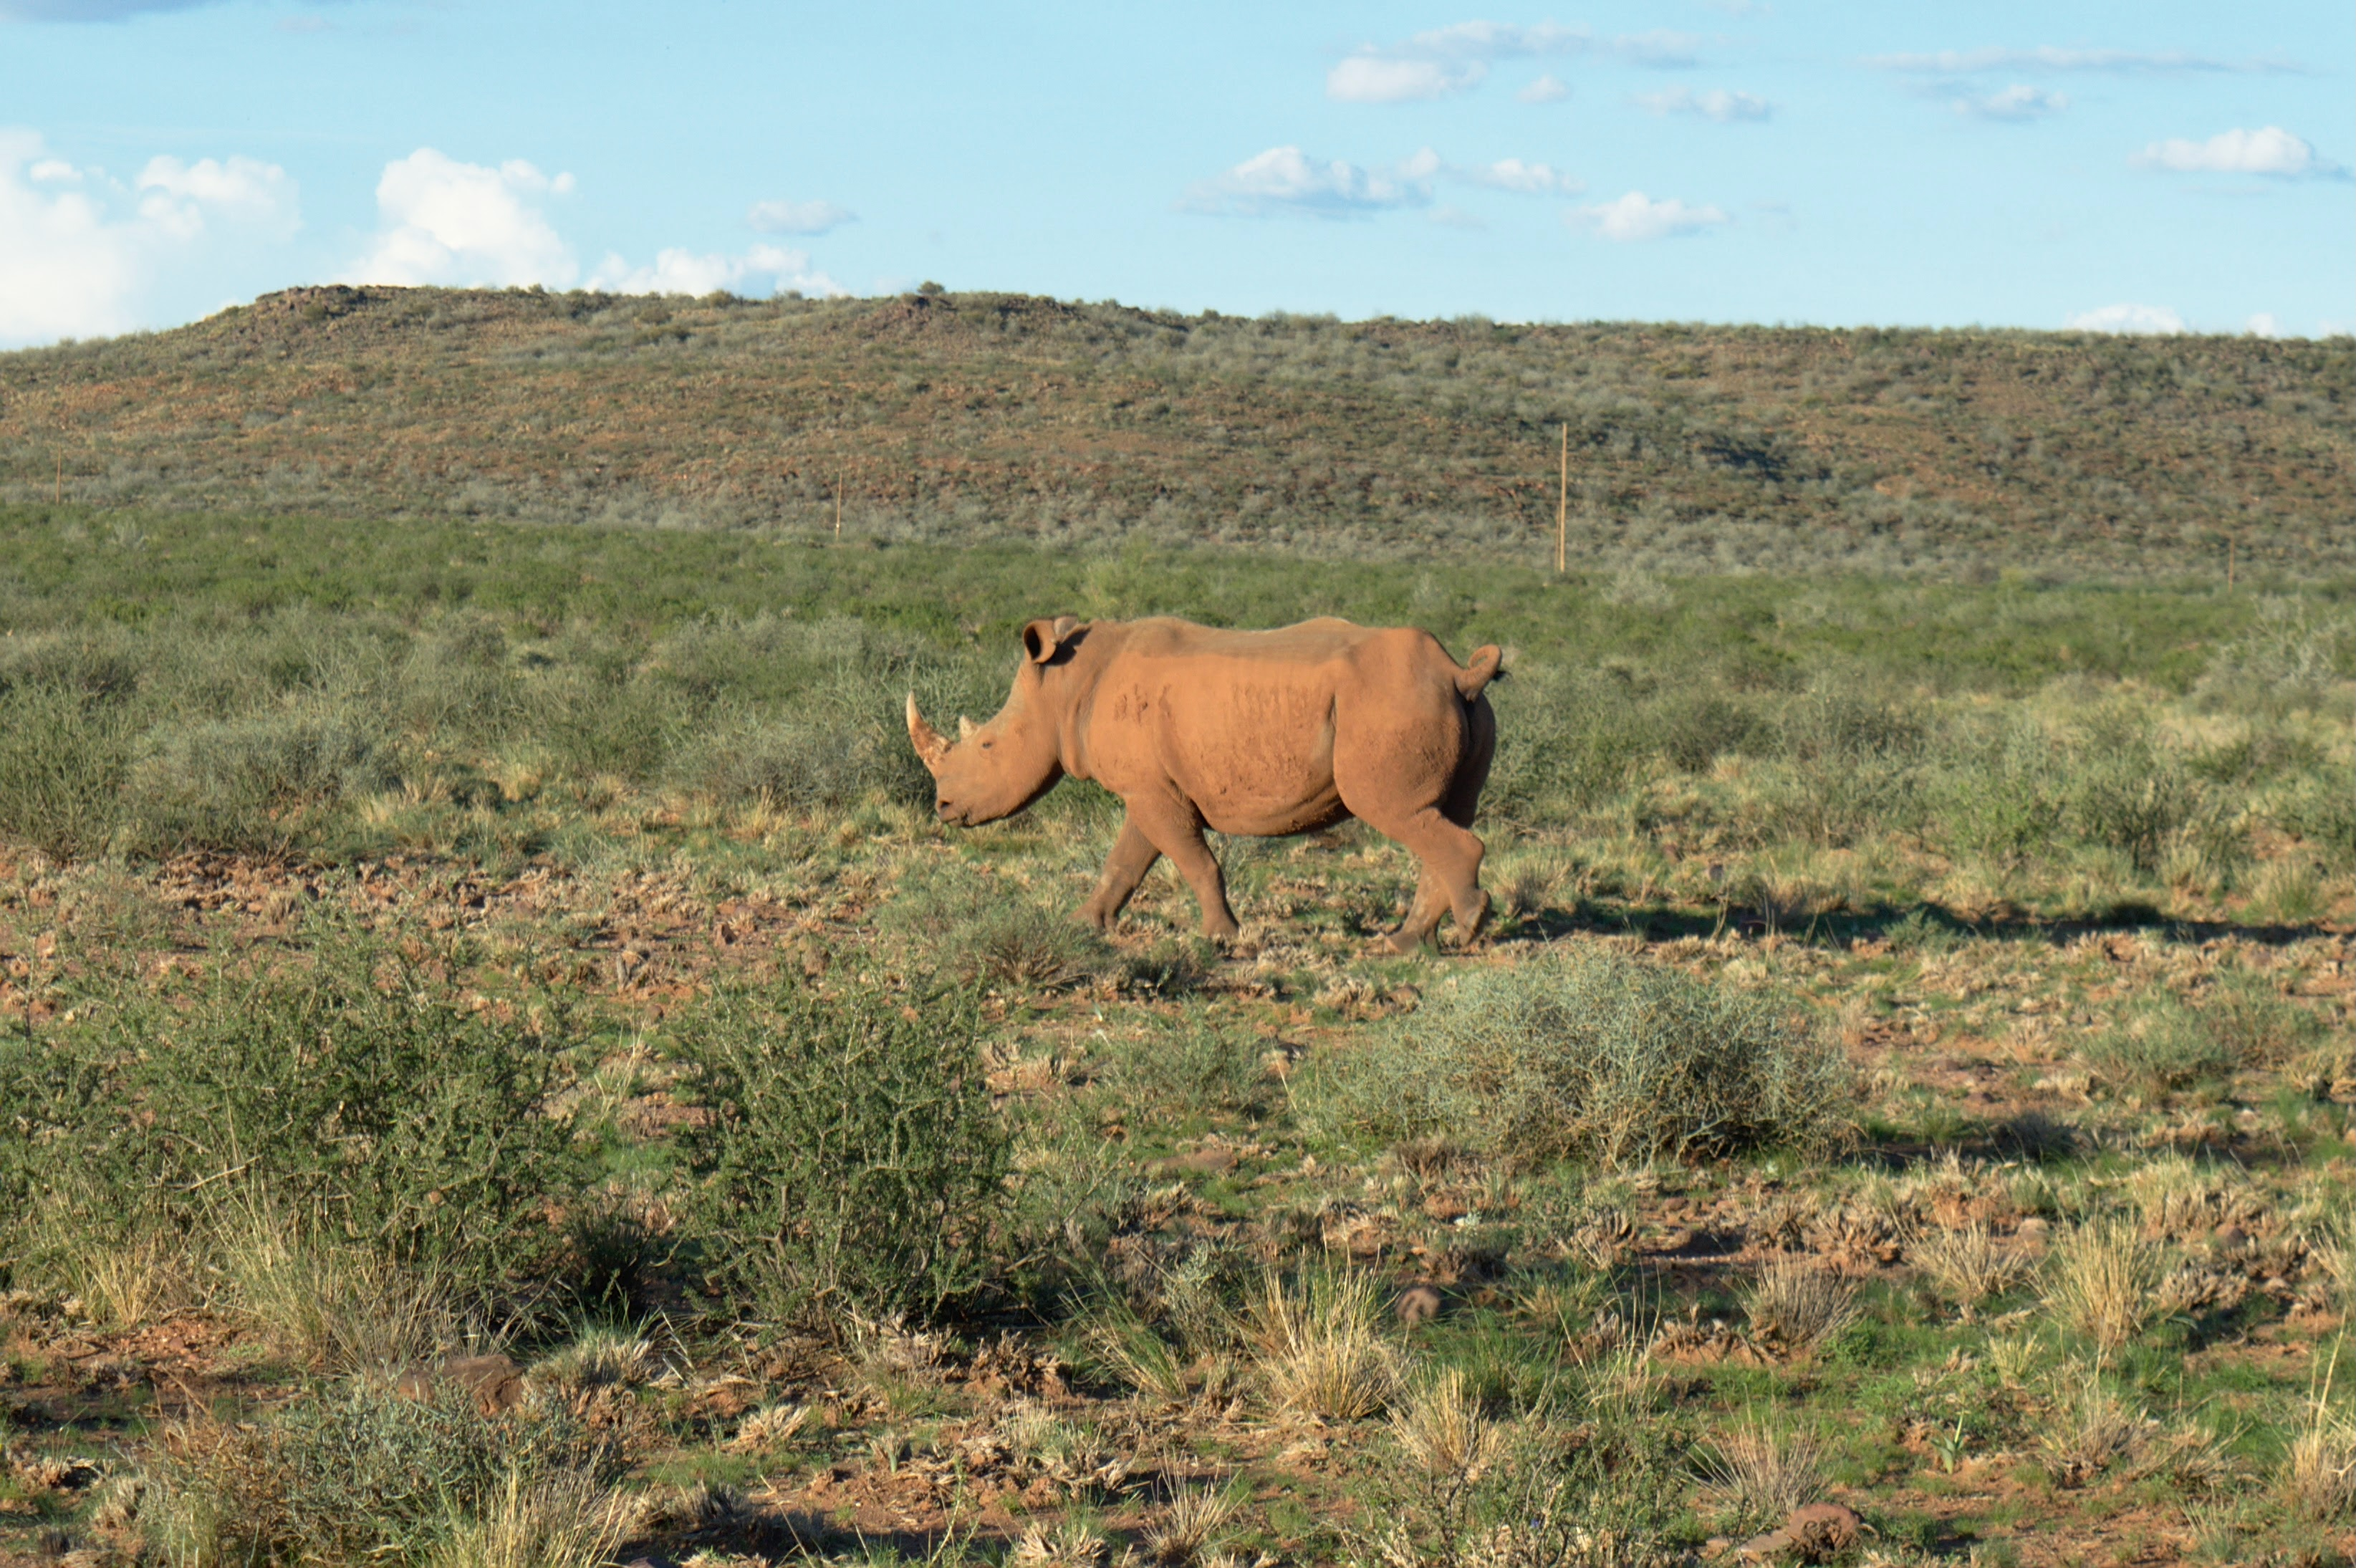
\includegraphics[width=.6\textwidth]{./static/rhino.jpg}
}

\note{
    There are numerous examples of applications of evolutionary game theory. In
    this particular paper, my co-authors and I modelled the practice of
    devaluing a Rhino's horn (either by dying it or cutting it off) to dissuade
    poachers.

    The logic behind this idea is that there is a best response by poachers
    which is to not kill a Rhino for its horn. However, using evolutionary game
    theory lets us understand if this is actually likely to happen.
}


\frame{
    \begin{center}
        \huge
        \url{nashpy.readthedocs.io}

        \url{knightva@cardiff.ac.uk}
    \end{center}
}

\end{document}
